\documentclass[10pt]{article}

\usepackage{fullpage}
\usepackage{setspace}
\usepackage{parskip}
\usepackage{titlesec}
\usepackage[section]{placeins}
\usepackage{xcolor}
\usepackage{breakcites}
\usepackage{lineno}
\usepackage{hyphenat}





\PassOptionsToPackage{hyphens}{url}
\usepackage[colorlinks = true,
            linkcolor = blue,
            urlcolor  = blue,
            citecolor = blue,
            anchorcolor = blue]{hyperref}
\usepackage{etoolbox}
\makeatletter
\patchcmd\@combinedblfloats{\box\@outputbox}{\unvbox\@outputbox}{}{%
  \errmessage{\noexpand\@combinedblfloats could not be patched}%
}%
\makeatother


\usepackage[round]{natbib}
\let\cite\citep




\renewenvironment{abstract}
  {{\bfseries\noindent{\abstractname}\par\nobreak}\footnotesize}
  {\bigskip}

\titlespacing{\section}{0pt}{*3}{*1}
\titlespacing{\subsection}{0pt}{*2}{*0.5}
\titlespacing{\subsubsection}{0pt}{*1.5}{0pt}


\usepackage{authblk}


\usepackage{graphicx}
\usepackage[space]{grffile}
\usepackage{latexsym}
\usepackage{textcomp}
\usepackage{longtable}
\usepackage{tabulary}
\usepackage{booktabs,array,multirow}
\usepackage{amsfonts,amsmath,amssymb}
\providecommand\citet{\cite}
\providecommand\citep{\cite}
\providecommand\citealt{\cite}
% You can conditionalize code for latexml or normal latex using this.
\newif\iflatexml\latexmlfalse
\AtBeginDocument{\DeclareGraphicsExtensions{.pdf,.PDF,.eps,.EPS,.png,.PNG,.tif,.TIF,.jpg,.JPG,.jpeg,.JPEG}}

\usepackage[utf8]{inputenc}
\usepackage[ngerman,english]{babel}










\begin{document}

\title{Feedback for AMO experimentalists}



\author[1]{Kai-Niklas S}%
\author[1]{apoorva.hegde}%
\author[1]{Andy Xia}%
\author[1]{Fred Jendrzejewski}%
\affil[1]{Kirchhoff-Institut für Physik}%


\vspace{-1em}



  \date{\today}


\begingroup
\let\center\flushleft
\let\endcenter\endflushleft
\maketitle
\endgroup








\sloppy


\section{Introduction}

We would like to control our system. And we will walk through this control by two examples.

\begin{enumerate}
\item The case of the intensity control, which is a very straight-forward example, which allows us to understand the basics.
\item A laser lock, which is less obvious as it is typically much less stable.
\end{enumerate}

\subsection{Terminology and Basics}
This section closely follow ideas from \cite{Bechhoefer_2005}. \newline
A generic feedback control is seen in Fig. \ref{195696}. A system G(s) is being controlled with a control signal r(s). The goal of the feedback is for the output of the system y(s) to follow the control signal r(s). The general idea is the following: measure the output of the system, determine its difference to the control voltage to get error $\epsilon$ and use this error signal as input for some control law K(s) that tries to minimize the error signal.

Here we analyze the system in frequency space, where $s=i\omega$. This is a convenient way to analyze control systems.   \newline
An easy way to measure quantity of such a system is the closed-loop transfer function $T$:
\begin{equation}
T= \frac{y(s)}{r(s)} = \frac{K(s)G(s)}{1+K(s)G(s)}
\end{equation}
For system stability the loop-shape \textit{H} is important and can be determined from \textit{T}:
\begin{equation}
H = K(s)G(s) = \frac{T}{1-T}
\end{equation}
Why? As we see from (1), the system gets unstable if $KG= -1$. This means that a feedback system will get unstable if $|KG|=1$ with a simultaneous phase lag of 180\selectlanguage{ngerman}°.\selectlanguage{english}
\begin{figure}[h!]
\begin{center}
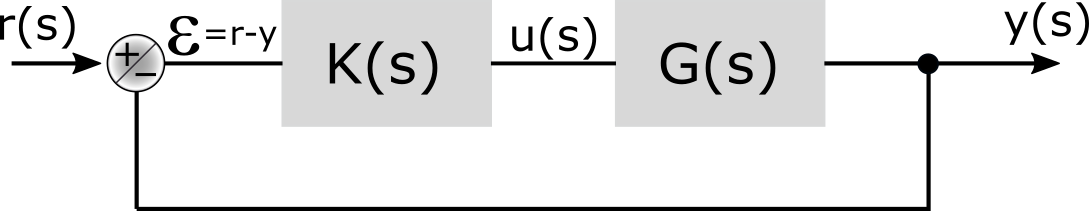
\includegraphics[width=0.42\columnwidth]{figures/text10419-5/text10419-5}
\caption{{Block diagram showing a generic feedback control. The system G(s) is
controlled by the control law K(s).
{\label{195696}}%
}}
\end{center}
\end{figure}

Whereas it is good to have control over an output variable up to a certain frequency, we are in many cases also interested in noise suppression. For example, atoms in a dipole trap experience a heating rate proportional to intensity fluctuations at twice the trap frequency. Only by suppressing the laser intensity noise, you can assure long trap lifetimes and/or ground state atoms. \newline
For this reason we consider output disturbances $d(s)$ and sensor noise $\xi (s)$ (see Fig. \ref{408256}):
\begin{equation}
y(s) = \frac{KG}{1+KG}[ r(s)-\xi(s)] + \frac{1}{1+KG}d(s)
\end{equation}
What does this mean? There are two things to learn from that. Let's start with the disturbances, and introduce the sensitivity, sometimes also called noise suppression:
\begin{equation}
S = \frac{1}{1+KG} = 1-T
\end{equation}
We see that a servo with a high gain leads to a low sensitivity to outside disturbances. \newline
The trade-off is that the higher the gain, the noisier the output signal. The reason is that with detector noise the control signal effectively becomes $r(s)-\xi(s)$, meaning that we cannot distinguish the control signal from measurement noise. Thus the higher the gain, the noisier the output.\selectlanguage{english}
\begin{figure}[h!]
\begin{center}
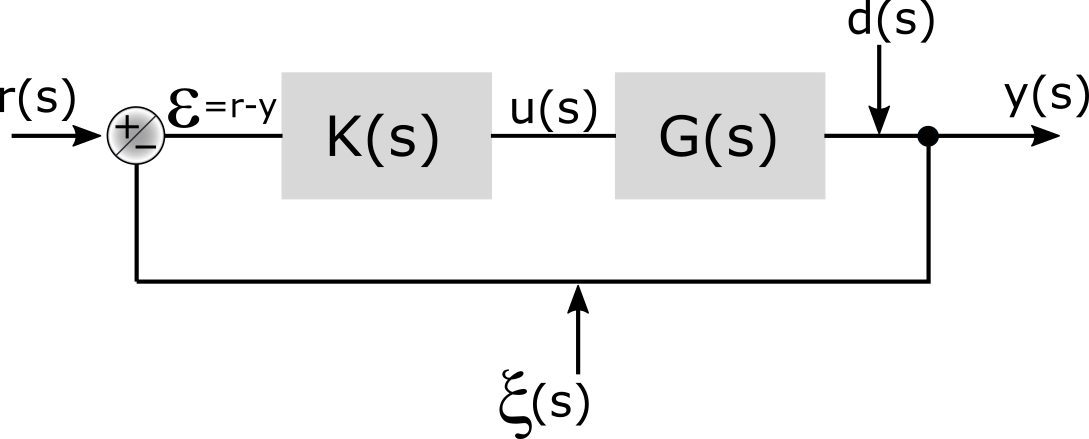
\includegraphics[width=0.42\columnwidth]{figures/path3909/path3909}
\caption{{Same system as Fig.{\ref{195696}}, but added
disturbances d(s) and detector noise.
{\label{408256}}%
}}
\end{center}
\end{figure}

Another trade-off - which holds for almost all systems (to be exact: if KG has at least two more poles than zeros, and has no poles in the right half plane (is stable)) - is the following:
\begin{equation}
\int_0^\infty ln|S(s)|ds =0
\end{equation}
This is known as Bode's sensitivity integral. It means that if you suppress the Sensitivity to disturbances in some frequency regime, you necessarily increase it in some other frequency regime (see Fig. \ref{840965} ).\selectlanguage{english}
\begin{figure}[h!]
\begin{center}
\includegraphics[width=0.42\columnwidth]{figures/slide-51/slide-51}
\caption{{If the Sensitivity to disturbances is suppressed in the low frequency
regime, it is necessarily increased in some higher frequency regime.
From \protect\cite{Stein_2003}
{\label{840965}}%
}}
\end{center}
\end{figure}

Now before looking at the different systems G(s), we have a look at the control law K(s). The most-used controller is the PID-controller, or very often experimentally only a PI-controller. The P stands for proportional gain, the I for integral gain and the D for derivative gain. Which makes sense if we look at the response in time domain:

\begin{equation}
u(t) = K_p\epsilon(t) + K_i\int \epsilon(t) dt + K_D \frac{d\epsilon}{dt}
\end{equation}

In frequency domain the same thing has the following form:

\begin{equation}
K(s) = \frac{u(s)}{\epsilon(s)} = K_p + \frac{K_i}{s} + K_Ds
\end{equation}


\section{Intensity stabilization}\label{intensity-stabilization}

\subsection{Overview}\label{overview}

For the control of the intensity, we typically have the set-up that is
sketched in Fig. \ref{685876}. The power of the AOM's first order beam
is dependent on the RF power: \(\epsilon_{1st order}\approx\sin^2(P_{RF}/P_{RF_{sat}})\). Therefore the power of
the laser beam that leads to the experiment can be controlled by
modulating the RF power.\selectlanguage{english}
\begin{figure}[h!]
\begin{center}
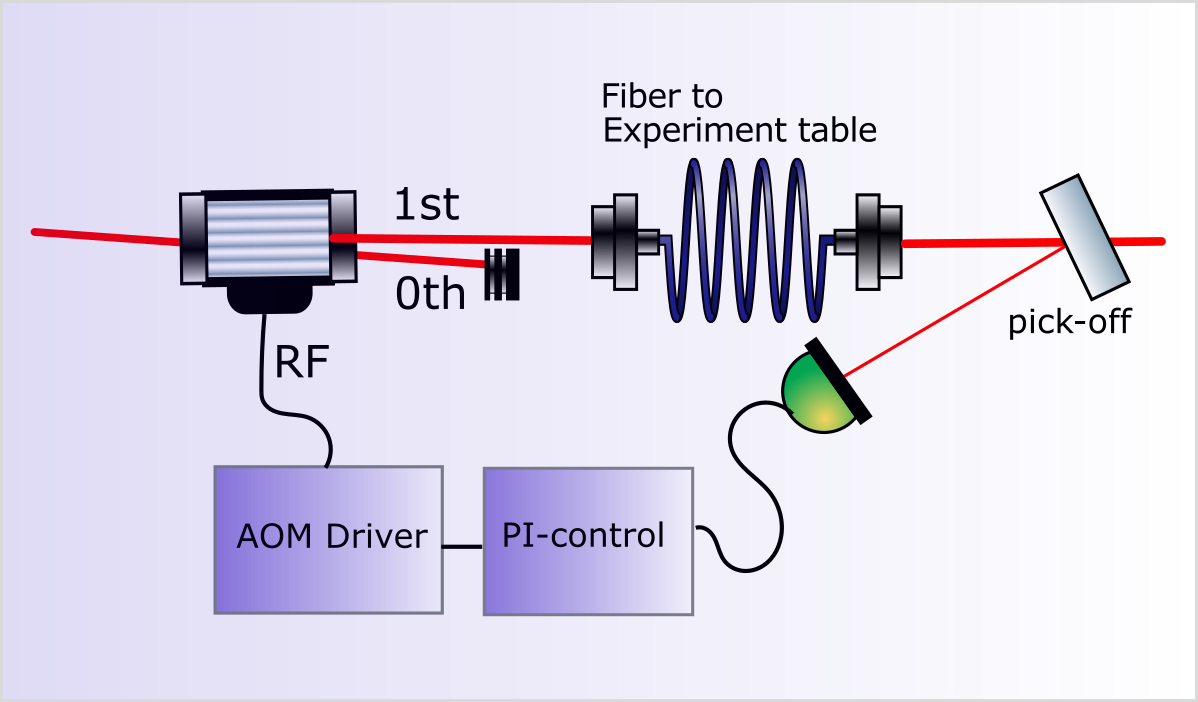
\includegraphics[width=0.42\columnwidth]{figures/rect14858/rect14858}
\caption{{A photodiode gets a fraction of the first order AOM beam. The Power of
this beam can be modulated via RF amplitude modulation.~
{\label{685876}}%
}}
\end{center}
\end{figure}

\subsection{The System}\label{the-system}

How to characterize the system without PI contol? (``system'' refers to
AOM+Driver+AOM+Photodiode) The tools needed for that are a function
generator, oscilloscope and a network analyzer. All of that can be found
in the RedPitaya we use (see Fig.
\ref{419186},\cite{pitaya},\cite{pyrpl}.\selectlanguage{english}
\begin{figure}[h!]
\begin{center}
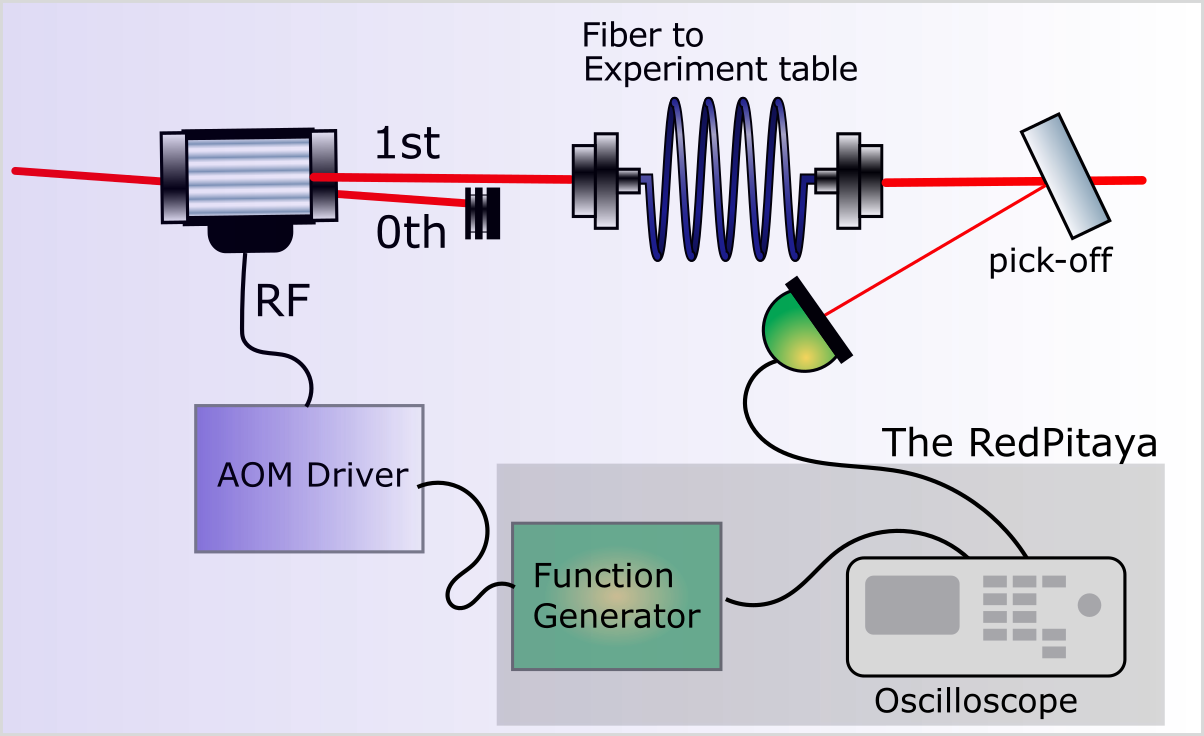
\includegraphics[width=0.42\columnwidth]{figures/text9831/text9831}
\caption{{This shows how to characetrize the system without PI-controller. The AOM
Driver expects a signal from 0 to 1V to attenuate the RF signal
accordingly. This again changes the 1st order beam power and therefore
the voltage on the photodiode. The RedPitaya can supply the control
voltage for the driver as well as measure the signal on the photodiode.
{\label{419186}}%
}}
\end{center}
\end{figure}



So what do we measure? As mentioned in the Introduction, we can measure
the closed-loop transfer function T (equation (1)) and then calculate
the open-loop transfer function H (equation (2)) to look for a desired
loopshape. \#\#\# How to change laser power by modulating RF power

The whole intensity stabilization is based on being able to modulate the
RF power that goes to the AOM. In our case, we have a home-build AOM
driver that allows for this modulation with a control voltage ranging
from 0 to 1V. Most drivers work with a Voltage Controlled Oscillator, a
Mixer or Variable Voltage Attenuator to attenuate the RF power, and and
an amplifier end-stage, because the AOM usually requires 30dBm, while
the VCO outputs something much lower.

Therefore the voltage on the photodiode depends on the control voltage
at the AOM driver and the dependency is nonlinear (see Figures
\ref{646448},\ref{747788}).\selectlanguage{english}
\begin{figure}[h!]
\begin{center}
\includegraphics[width=0.70\columnwidth]{figures/nonlinearity/Oscilloscope-trace}
\caption{{Scope trace: The control voltage of the aom driver in orange, the
corresponding photodiode signal in blue
{\label{646448}}%
}}
\end{center}
\end{figure}\selectlanguage{english}
\begin{figure}[h!]
\begin{center}
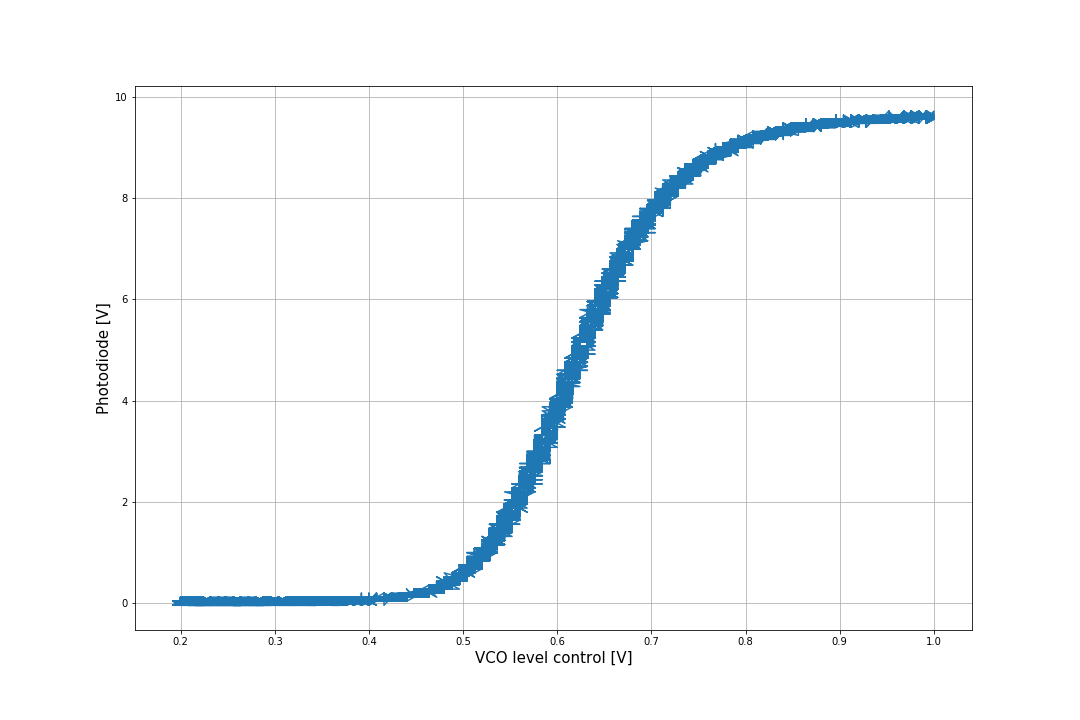
\includegraphics[width=0.70\columnwidth]{figures/Oscilloscope-trace/nonlinearity}
\caption{{Relationship between control voltage and photodiode voltage. Not that
the y-axis is basically arbitrary, as this depends on pick-off ratio and
initial laser power.
{\label{747788}}%
}}
\end{center}
\end{figure}

\subsubsection{Analysis in Frequency space with Bode
plots}\label{analysis-in-frequency-space-with-bode-plots}

The RedPitaya with its network analyzer module, allows us to
characterize the setup in frequency space. In Fig. \ref{747788} we saw
how the Photodiode voltage (laser power) depends on the control voltage
on the AOM driver when applying a DC or very low frequency signal. Now
we modulate the VCO control voltage with the following:
\(U_{control}=0.6V+0.01V\cdot\sin\left(2\cdot\pi\cdot f\cdot t\right)\) Can the Photodiode follow this modulation up to
arbitrary frequency? Probably not, but how can we measure this? The
network analyzer can excite the system with above voltage
\(U_{control}\) and compare the amplitude of oscillation in the and
\(U_{Photodiode}\) to measure magnitude and phase. It does so by
demodulating the photodiode signal with the same sine that was used for
excitation and a corresponding cosine, then lowpass-filtering and
averaging the two quadratures for a well-defined number of cycles (see
Pyrpl API). From the two quadratures it is now possible to extract the
magnitude and phase shift of our system in the probed frequency regime
(see Figure \ref{852375}). In Figure \ref{852375} we see that for low
frequencies the system follows without phase lag and for higher
frequencies the phase increasingly lags as the signal magnitude
decreases.\selectlanguage{english}
\begin{figure}[h!]
\begin{center}
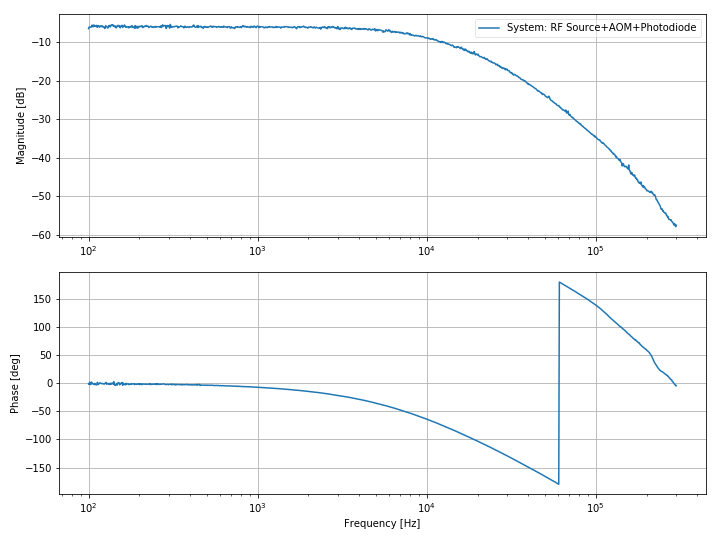
\includegraphics[width=0.70\columnwidth]{figures/System-RF-Source+AOM+Photodiode/System-RF-Source+AOM+Photodiode}
\caption{{System Transfer Function: Obtained by modulating the RF attenuation of
the AOM driver with different frequencies and measuring the
corresponding signal on the Photodiode.~ Do not get confused by
the~\emph{absolute~}Magnitude of the Gain values: A sinusoidal signal
with 1mV amplitude going into the AOM driver does~\emph{not~}correspond
to a signal with 1mV on the photodiode. This is for example dependent on
the offset (because of the slope) or the photodiode amplification.
The~\emph{relative~}numbers however give you insight in attenuation at
higher frequencies and therefore System bandwidth.
{\label{852375}}%
}}
\end{center}
\end{figure}

\subsection{The control law}\label{the-control-law}\selectlanguage{english}
\begin{figure}[h!]
\begin{center}
\includegraphics[width=0.70\columnwidth]{figures/Controllaw/Controllaw}
\caption{{Measured control-laws of the RedPitaya. The red curve shows just a
P-controller, whereas the rest shows a PI-controller
{\label{569947}}%
}}
\end{center}
\end{figure}

\subsection{A closed loop}\label{a-closed-loop}

After connecting the PI-controller which in our case is also done by the
RedPitaya, we close the feedback loop (see Figure \ref{195696},
\ref{685876}). Now we select some proportional and integral constants
such that the intensity is locked to a setpoint we choose.\\
That means that the voltage on the photodetector will be the same as the
chosen setpoint.\\
How do we characterize the lock now? How do we know how stable the lock
is? How do we know until which frequency noise is surpressed? We take
the closed-loop transfer function \emph{T} using the RedPitaya (see
Figure \ref{852979}). With that we can calculate the open-loop transfer
function \emph{H} and look at the sensitivity \emph{S}.\selectlanguage{english}
\begin{figure}[h!]
\begin{center}
\includegraphics[width=0.70\columnwidth]{figures/Closed-loop-Transfer-function/Closed-loop-Transfer-function}
\caption{{Closed-loop transfer function T measured by the RedPitaya. For low
frequencies the photodiode voltage follows the modulation well. For
higher frequencies the gain of the system decreases. For higher
proportional constant the transfer function does not decrease as much at
higher frequencies.
{\label{852979}}%
}}
\end{center}
\end{figure}

\subsection{The open loop}\label{the-open-loop}

After measuring \emph{T} we can can calculate \emph{H} (see Figure
\ref{458024}).\\
As mentioned in the introduction the criterion for instability is
\(\left|H\right|>1\) for a simultaneously phase lag close to 180\selectlanguage{ngerman}°. Be
careful that the unit in the figure is dB, which means that
\(\left|H\right|= 1 = 0 dB\). For low frequencies the transfer functino is ruled
by the integrator's characteristics. Which means high gain, but only a
phase lag of 90°.\\
The interesting regime is where the phase lag hits -180\selectlanguage{ngerman}° which happens
for \textasciitilde{}40kHz for the orange curve and
\textasciitilde{}90kHz for the blue curve. But both sets of
P\&I-constants lead to stable behaviour, because the magnitude at that
point is below 0dB.\\
The conclusion of this analysis shows that we could have gotten away
with a higher proportional or integral constant and still have a stable
system.\selectlanguage{english}
\begin{figure}[h!]
\begin{center}
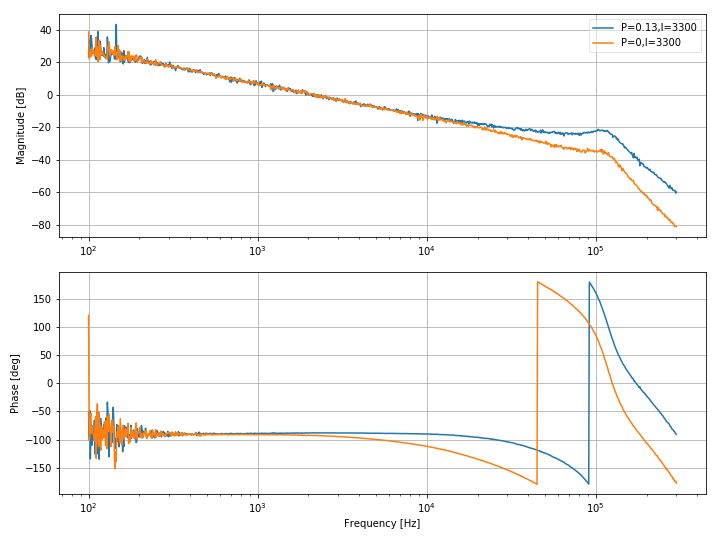
\includegraphics[width=0.70\columnwidth]{figures/Loop-Gain/Loop-Gain}
\caption{{Open-loop transfer function H.~
{\label{458024}}%
}}
\end{center}
\end{figure}

\subsection{Sensitivity and noise
surpression}\label{sensitivity-and-noise-surpression}\selectlanguage{english}
\begin{figure}[h!]
\begin{center}
\includegraphics[width=0.70\columnwidth]{figures/Noiseplot/Sensitivity-and-Loop-Gain}
\caption{{Open-loop transfer function and Sensitivity.
{\label{827693}}%
}}
\end{center}
\end{figure}\selectlanguage{english}
\begin{figure}[h!]
\begin{center}
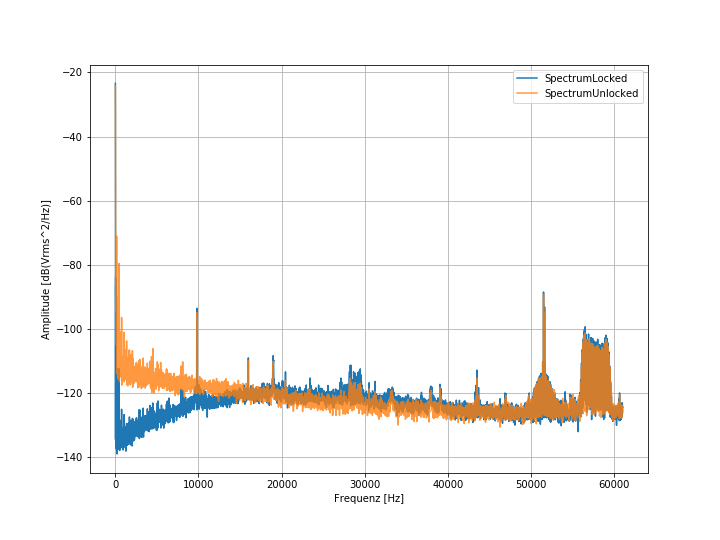
\includegraphics[width=0.70\columnwidth]{figures/Sensitivity-and-Loop-Gain/Noiseplot}
\caption{{Noise spectra locked and unlocked.~
{\label{334258}}%
}}
\end{center}
\end{figure}



\subsection{Further Reading: Problems of Intensity
stabilization}\label{further-reading-problems-of-intensity-stabilization}

Here we can already identify the first pitfall of intensity
stabilization. The system, mainly the attenuator inside of the AOM
driver, has a proportional gain that depends on the control voltage and
is proportional to the slope in Figure \ref{747788}. The highest gain
(slope) is around a control voltage of 0.6V, and the proportional gain
for values at 0.4V and 0.9V is very low. On the contrary, the
PI-controller has \emph{fixed} proportional and integral constants.\\
If you only want one specific laser power in your experiment, this does
not bother you. You are using more or less one control voltage that
gives you the desired laser power and then you tune the proportional
constant of your PI-controller such that the system has the biggest
bandwidth.\\
But imagine you would want to change this laser power now. By choosing a
different setpoint/control voltage you would increase/decrease your
proportional gain drastically end end up with an oscillating system or a
system with very low bandwidth. If you would want your system to be
stable for all control voltages, you would have to make sure that for
the highest system proportional gain for a control voltage of 0.6V, you
choose your PI-controller proportional gain such that your system is
stable. Then you have the biggest bandwidth around a control voltage of
0.6V, but for all other control voltages you would have a smaller
bandwidth. Imagine the worst case: You want high laser power for loading
your laser dipole trap, and then reduce the trap depth for evaporative
cooling by decreasing the laser power by a factor of 100. In Figure
\ref{747788} this could for example mean, that you have a photodiode
voltage of 9V for loading your trap and 90mV for evaporative cooling. In
both cases the slope (proportional gain) is very small. If you want your
laser power to be stable and not oscillating during the ramp-down
(decrease of factor 100), you would have to accept a low bandwidth in
both cases, for the loading and the evaporative cooling.\\
One work-around could be that you sacrifice system-stability during the
ramp-down for higher proportional gains in the loading and cooling
stage. This however could lead to atom-loss due to parametric heating.

Another thing to keep in mind: usually your experimental approach is the
following: I want 100mW during the first stage of the experiment and
10mW during the second stage of the experiment. For you to be able to
choose a good regime of control voltage values, e.g.~0.5-0.7V, where the
AOM Driver gain changes minimally, you have to be able to change either
photodiode gain, pick-off ratio or initial laser power.

\subsubsection{Frequency dependence}\label{frequency-dependence}

The AOM Driver expects an input of 0-1V for modulating the RF Power (see
Fig. \ref{639282}). For characterizing the response of the system at
different frequencies, you choose an offset, e.g.~600mV. Then you
modulate this with a sine with small amplitude (small enough that the
nonlinear behaviour of the Driver characteristics (see Fig.
\ref{639282}) are approximately linear) and look at the corresponding
photodiode signal. You are interested in what the photodiode signal
looks at different frequency modulations. This is exactly what a network
analyzer does, a tool that is also included in the RedPitaya. The result
of this measurement can be summarized in a Bode plot (see Fig.
\ref{303565}).

It's clear that this system doesn't have any resonances and behaves
quiet nicely in the displayed frequency regime. Therefore time-domain
tuning methods for a servo like Ziegler-Nichols tuning can be effective
and quick. But not every system behaves as nicely as this, so looking at
the frequency-regime can be interesting and a way to improve your
control, e.g.~finding and filtering resonances makes it possible to
increase overall gain without sacrificing stability.

\selectlanguage{english}
\FloatBarrier
\bibliographystyle{plainnat}
\bibliography{bibliography/converted_to_latex.bib%
}

\end{document}

